\documentclass[11pt]{article}


\usepackage{amsfonts}
\usepackage{fancyvrb}
\usepackage{graphicx}
\usepackage{caption}
\usepackage{subcaption}
\usepackage{url}

\setlength{\oddsidemargin}{0in}
\setlength{\evensidemargin}{0in}
\setlength{\textwidth}{6.5in}
\setlength{\topmargin}{0in}
\setlength{\headsep}{0.5in}
\setlength{\textheight}{8.5in}
\setcounter{page}{1}
%\pagestyle{empty}
%\hbadness=10000

\begin{document}
\huge
\noindent
{Discrete Optimization Assignment:}
\vspace{0.25cm}

\noindent
{\bf Vehicle Routing}
\normalsize


\section{Problem Statement}


In this assignment you will design an algorithm to solve a problem faced by package delivery companies, {\em The Vehicle Routing Problem (VRP)}.  Every day, a delivery company needs to deliver goods to many different customers.  The deliveries are achieved by dispatching a fleet of vehicles from a centralized storage warehouse.  The goal of this problem is to design a route for each vehicle (similar to traveling salesman tours) so that all of the customers are served by exactly one vehicle and the travel distance of the vehicles is minimized.  Additional problem complexity comes from the fact that the vehicles have a fixed storage capacity and the customers have different demands.  Figure \ref{fig:vrp} illustrates a small VRP and a feasible solution to that problem.  The customers are labeled from $0$ to $4$, with $0$ being the warehouse.  The solution uses two vehicles which are indicated by different colored routes.


\begin{figure}[h]
        \centering
        \begin{subfigure}[b]{8.0cm}%{0.3\textwidth}
                \centering
                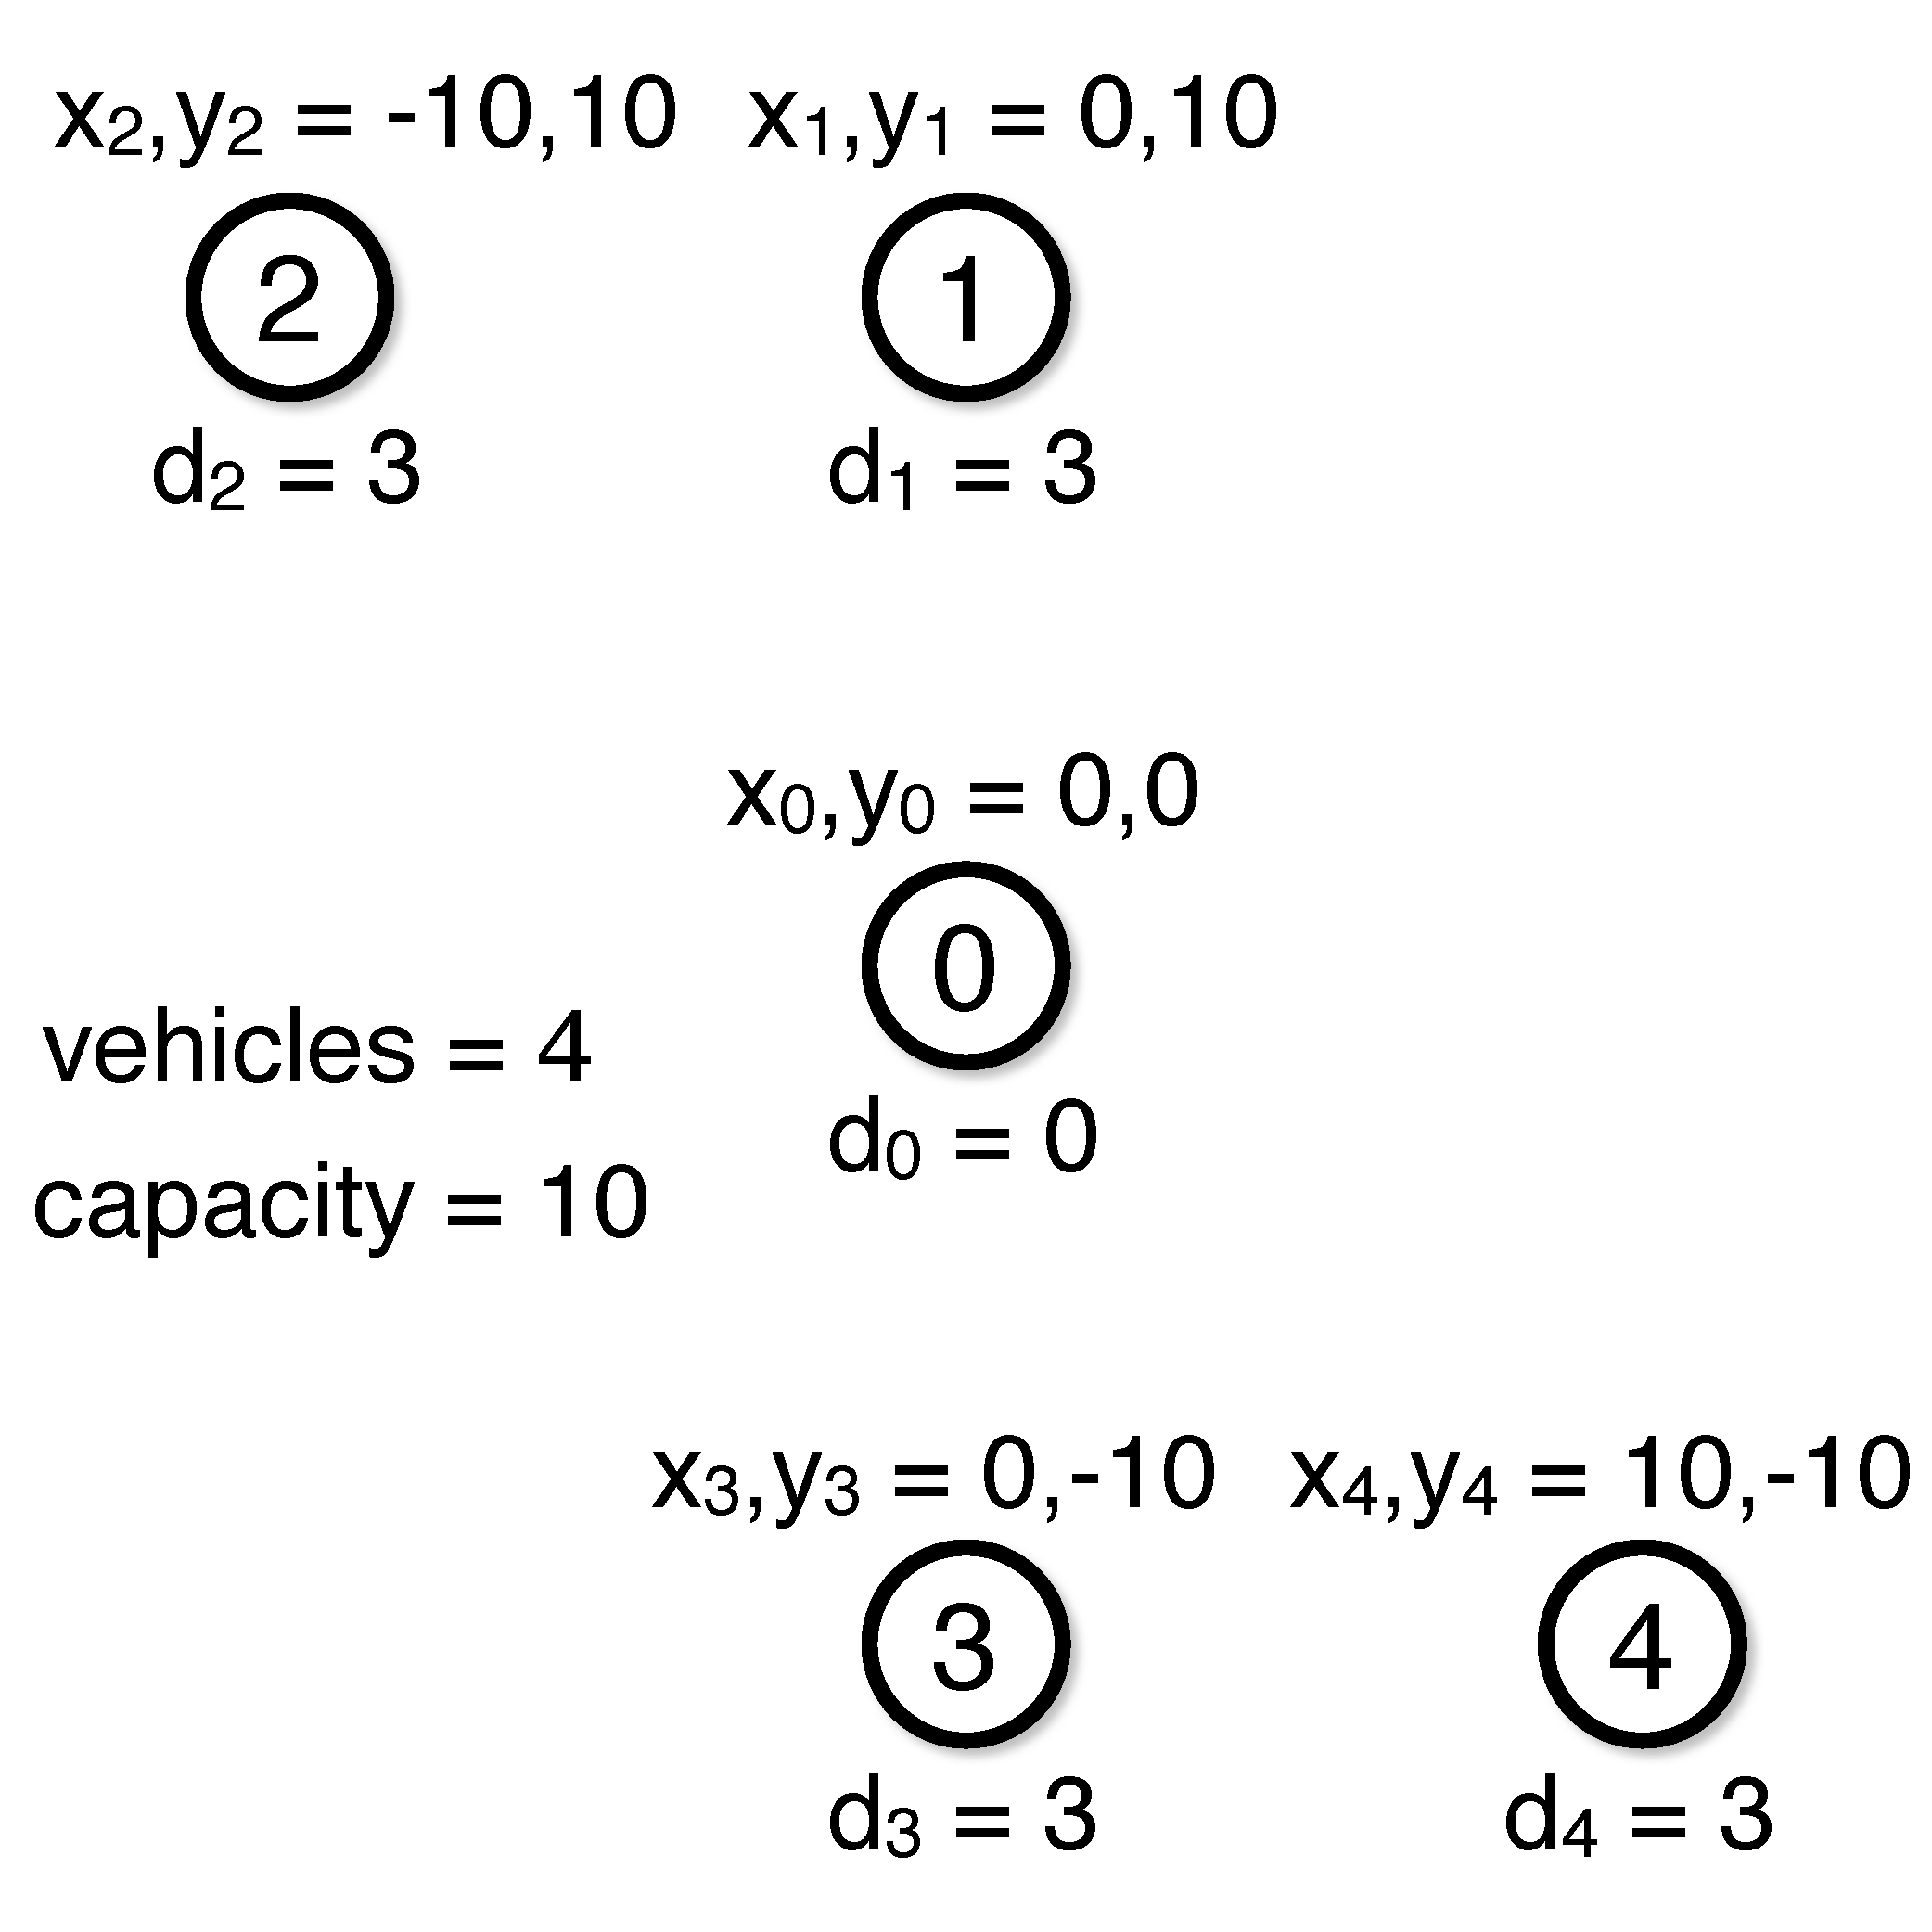
\includegraphics[width=6cm]{figures/vrp_1.pdf}
                \caption{The VRP input data.}
                \label{fig:vrp:input}
        \end{subfigure}%
        ~ %add desired spacing between images, e. g. ~, \quad, \qquad etc.
          %(or a blank line to force the subfigure onto a new line)
        \hfill
        \begin{subfigure}[b]{8.0cm}
                \centering
                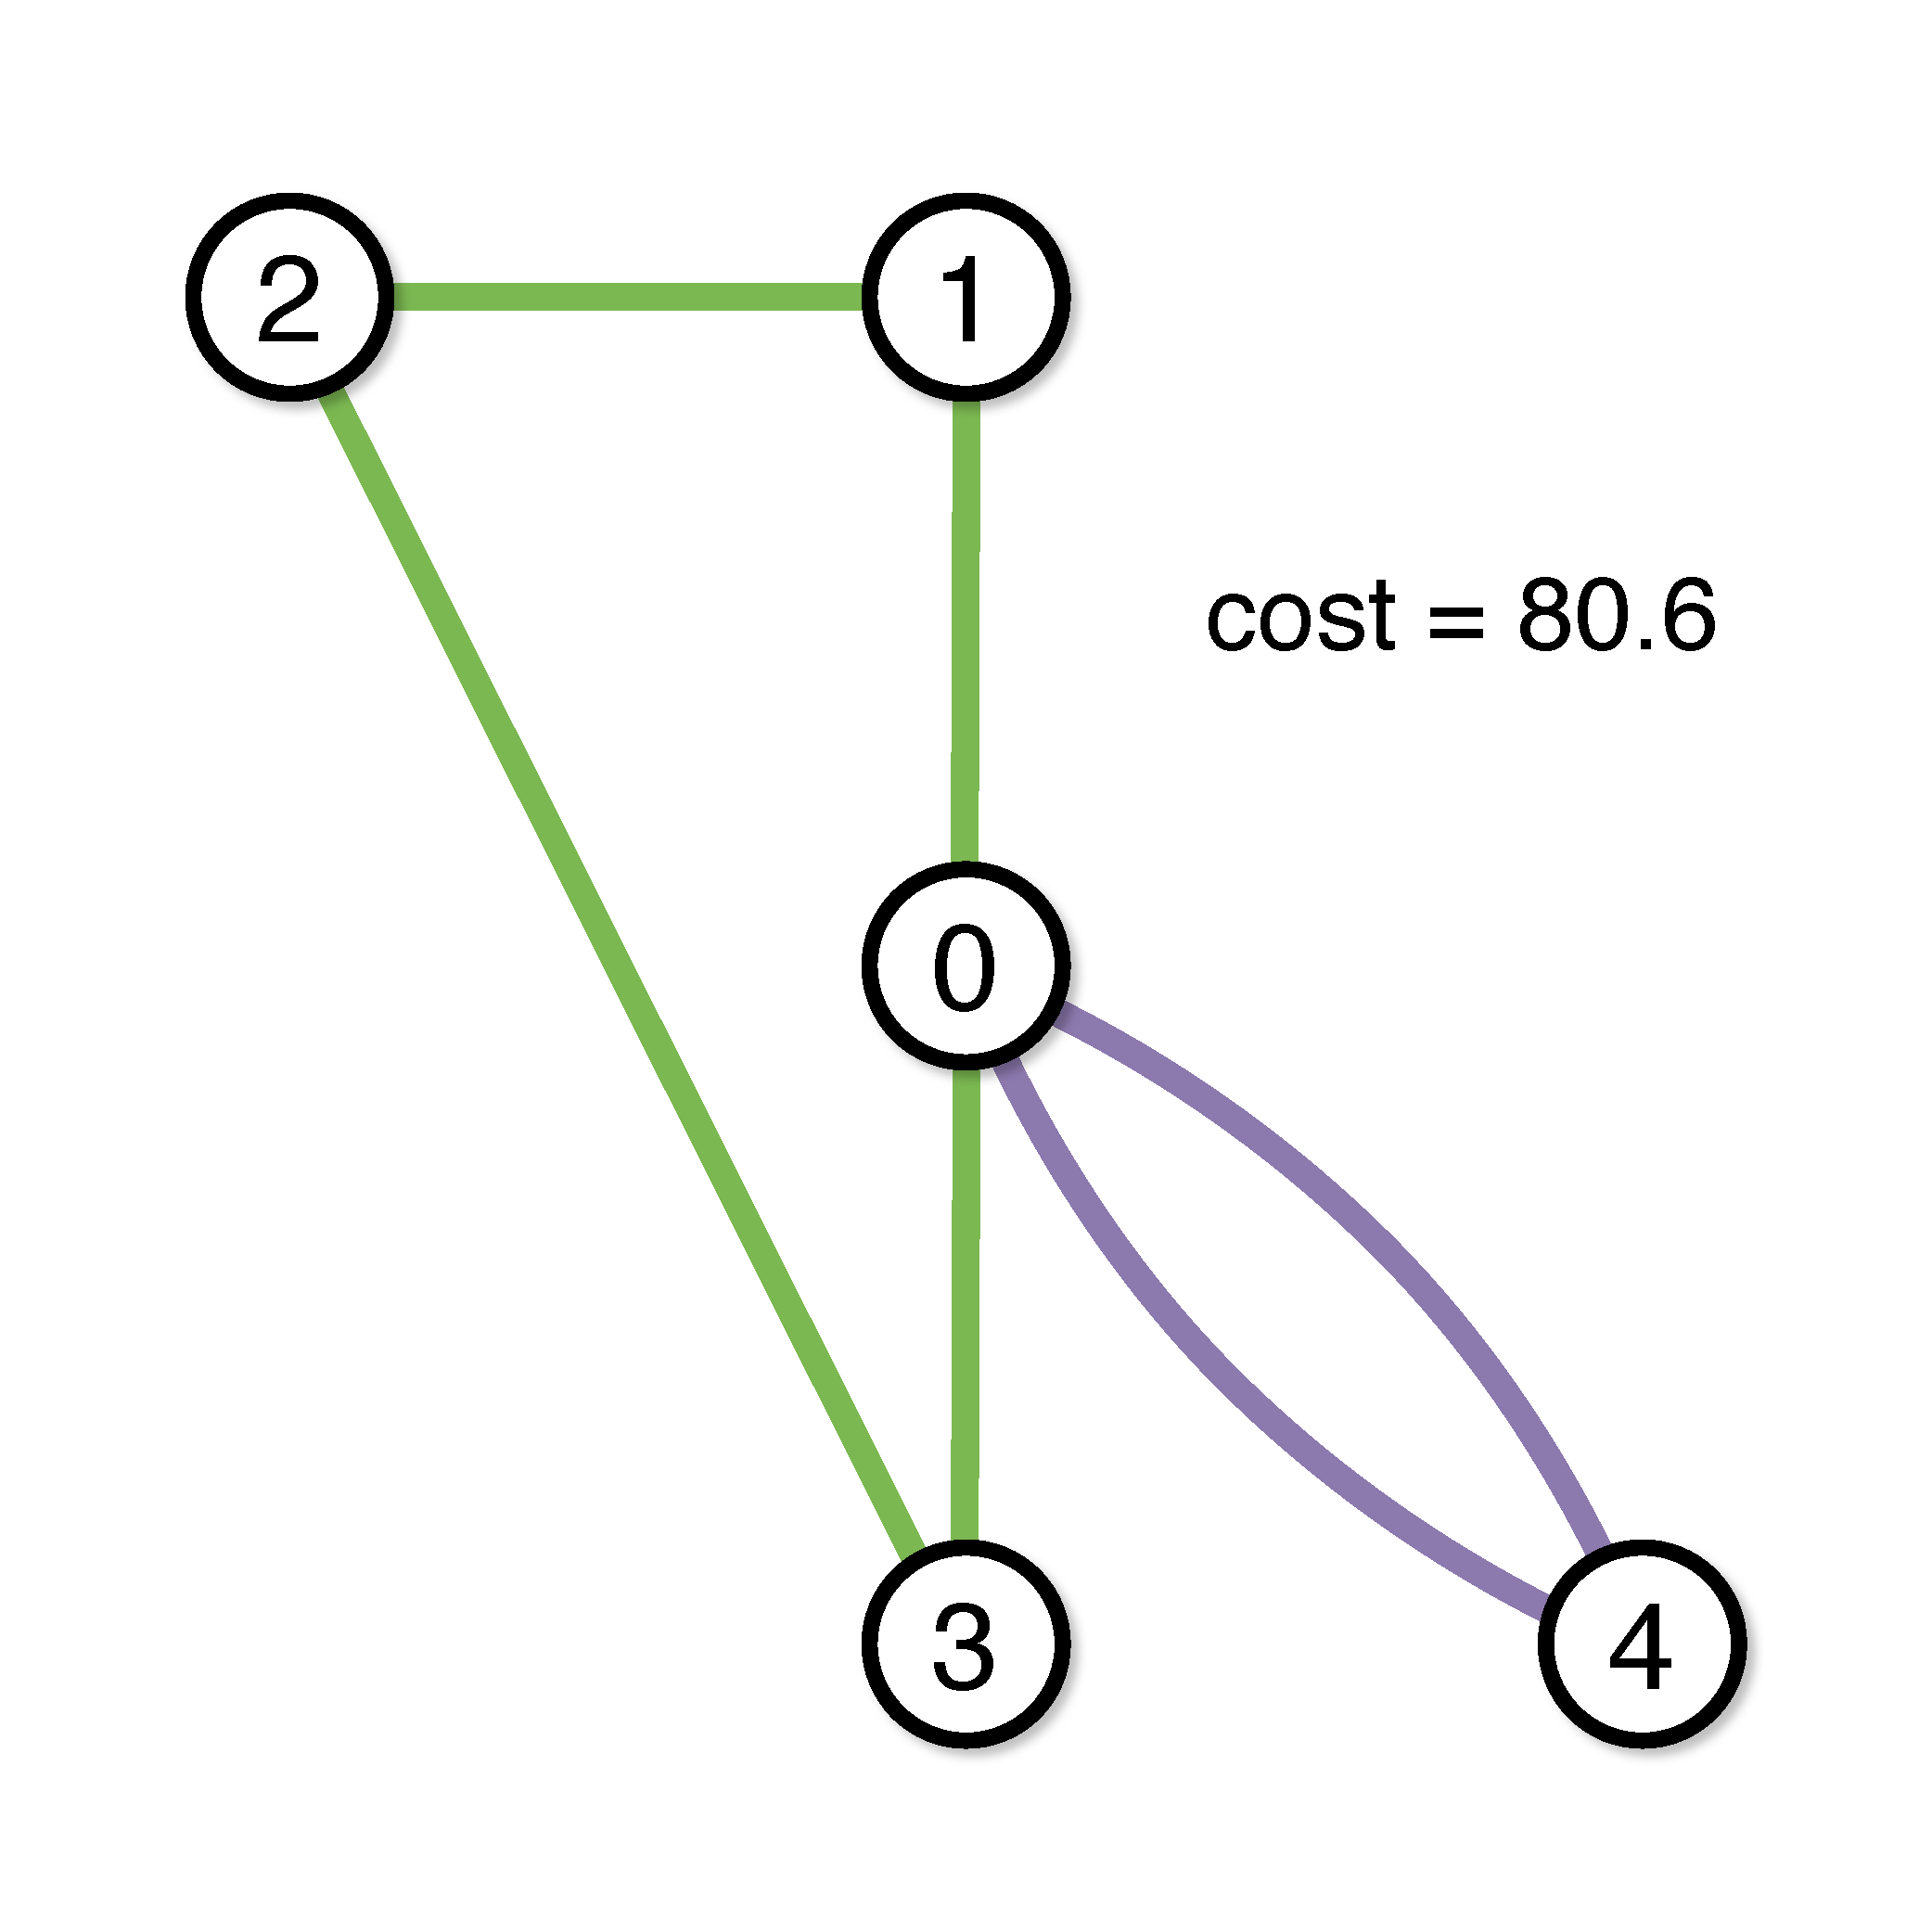
\includegraphics[width=6cm]{figures/vrp_2.pdf}
                \caption{A solution to the VRP using 2 vehicles.}
                \label{fig:vrp:sol}
        \end{subfigure}
        \caption{A Vehicle Routing Example}\label{fig:vrp}
\end{figure}

\section{Assignment}

Write an algorithm to solve the vehicle routing problem.  The problem is mathematically formulated in the following way:  We are given a list of locations $N = 0 \ldots n-1$.  By convention, location 0 is the warehouse location, where all of the vehicles start and end their routes.  The remaining locations are customers.  Each location is characterized by three values  $\langle d_i,x_i,y_i \rangle \; i \in N$ a demand $d_i$ and a point $x_i,y_i$.  The fleet of vehicles $V = 0 \ldots v-1$ is fixed and each vehicle has a limited capacity $c$.  All of the demands assigned to a vehicle cannot exceed its capacity $c$.  For each vehicle $i \in V$, let $T_i$ be the sequence of customer deliveries made by that vehicle and let ${\it dist}(c_1,c_2)$ be the Euclidean distance between two customers.\footnote{${\it dist}(j,k) = \sqrt{(x_{j} - x_{k})^2 + (y_{j} - y_{k})^2}$}  Then the vehicle routing problem is formalized as the following optimization problem,
$$
\begin{array}{ll}
\mbox{minimize:} & \displaystyle \sum_{i \in V} \left( dist(0, T_{i,0}) + \sum_{\langle j,k \rangle \in T_{i}} dist(j, k) + dist(T_{i,|T_i|-1}, 0) \right)\\
\mbox{subject to:} & \\
     & \displaystyle \sum_{j \in T_{i}} d_j \leq c \;\;\; (i \in V) \\
     & \displaystyle \sum_{i \in V}  (j \in T_{i}) = 1 \;\;\; (j \in N \setminus 0) 
\end{array}
$$
In this variant of the vehicle routing problem, we assume the vehicles can travel in straight lines between each pair of locations.

\section{Data Format Specification}

The input consists of $|N| + 1$ lines.  The first line contains 3 numbers: The number of customers $|N|$, the number of vehicles $|V|$, and the vehicle capacity $c$.
It is followed by $|N|$ lines, each line represents a location triple $\langle d_i,x_i, y_i \rangle$, with a demand $d_i \in \mathbb{N}$ and a point  $x_i, y_j \in \mathbb{R}$.

\vspace{0.2cm}
\noindent
Input Format
\vspace{-0.2cm}
\begin{Verbatim}[frame=single]
|N| |V| c
d_0 x_0 y_0
d_1 x_1 y_1
...
d_|N|-1 x_|N|-1 y_|N|-1
\end{Verbatim}
%
The output has $|V|+1$ lines.  The first line contains two values $obj$ and $opt$.  $obj$ is the length of all of the vehicle routes (i.e. the objective value) as a real number.  $opt$ should be $1$ if your algorithm proved optimality and $0$ otherwise.  The following $|V|$ lines represent the vehicle routes $T$ encoding the solution.  Each vehicle line starts with warehouse identifier $0$ followed by the identifiers of the customers serviced by that vehicle and ends with the warehouse identifier $0$.  Each vehicle line can contain between $2$ and $|N|+2$ values depending on how many customers that vehicle services.  Each customer identifier must appear in one of these vehicle lines.

\vspace{0.2cm}
\noindent
Output Format
\vspace{-0.2cm}
\begin{Verbatim}[frame=single]
obj opt
0 t_0_1 t_0_2 ... 0 
0 t_1_1 t_1_2 ... 0 
...
0 t_|V|-1_1 t_|V|-1_2 ... 0
\end{Verbatim}
%
%It is essential that the value order in the solution output matches the value order of the input.  Otherwise the grader will misinterpret the output.

\clearpage
\paragraph{Examples} \mbox{}
%\vspace{0.1cm}
\noindent
(based on Figure \ref{fig:vrp})

\vspace{0.2cm}
\noindent
Input Example
\vspace{-0.2cm}
\begin{Verbatim}[frame=single]
5 4 10
0 0 0
3 0 10
3 -10 10
3 0 -10
3 10 -10
\end{Verbatim}

\vspace{0.2cm}
\noindent
Output Example 1
\vspace{-0.2cm}
\begin{Verbatim}[frame=single]
80.6 0
0 1 2 3 0 
0 4 0
0 0
0 0
\end{Verbatim}
%
This output represents the following routes for each vehicle.  Vehicle 0 - $\{0 \rightarrow 1, 1 \rightarrow 2, 2 \rightarrow 3, 3 \rightarrow 0\}$;  Vehicle 1 - $\{0 \rightarrow 4, 4 \rightarrow 0\}$; Vehicle 2 - $\{0 \rightarrow 0\}$; Vehicle 3 - $\{0 \rightarrow 0\}$.  Note the following equivalent solution using the same routes with different vehicles.  

\vspace{0.2cm}
\noindent
Output Example 2
\vspace{-0.2cm}
\begin{Verbatim}[frame=single]
80.6 0
0 4 0
0 0
0 1 2 3 0 
0 0
\end{Verbatim}

\section{Instructions}

Edit \texttt{solver.py} and modify the \texttt{solve\_it(input\_data)} function to solve the optimization problem described above.  The function argument, \texttt{input\_data}, contains the problem data in the format described above.  The return value of \texttt{solve\_it} is a solution to the problem in the output format described above.  Your \texttt{solve\_it} implementation can be tested with the command, 
\[ 
\texttt{python ./solver.py ./data/<inputFileName>} 
\] 
You should limit the \texttt{solve\_it} method to terminate within 5 hours, otherwise the submission will not be eligible for full credit.  You may choose to implement your solver directly in python or modify the \texttt{solve\_it} function to call an external application.

%We use \texttt{stdout} for output.
%Output to other stream will be ignored (you may want to send runtime information to \texttt{stderr}). Your submission will be tested on a department linux machine. If your algorithm is a standalone program, please name it \texttt{nr},
%otherwise, please specify the compilation procedure,
%it is appreciated if you also provide a script that follows the above format to run the program.

\paragraph{Resources}
You will find several vehicle routing problem instances in the \texttt{data} directory provided with the handout.

%An example output file, \texttt{blabla.out}, is also provided.

%\section{Remarks}

\paragraph{Handin}
Run \texttt{submit.py} with the command, \texttt{python ./submit.py}.  Follow the instructions to apply your  \texttt{solve\_it} method on the various assignment parts.  You can submit multiple times and your grade will be the best of all submissions.  However, it may take several minutes before your assignment is graded; please be patient.  You can track the status of your submission on the {\em feedback} section of the assignment website.


\paragraph{Grading}
Infeasible solutions (i.e. those that do not conform to the output format or violate problem constraints) will receive 0 points.  Feasible solutions will receive at least 3 points.  Feasible solutions passing a low quality bar will receive at least 7 points and solutions meeting a high quality bar will receive all 10 points.  The grading feedback indicates how much your solution must improve to receive a higher grade.


\paragraph{Collaboration Rules} 

In all assignments we encourage collaboration and the exchange of ideas on the discussion forums.  However, please refrain from the following:
\begin{enumerate}
\item Posting code or pseudo-code related to the assignments.
\item Using code which is not your own.
\item Posting or sharing problem solutions.
\end{enumerate}
Discussion of solution quality (i.e. objective value) and algorithm performance (i.e. run time) is allowed and the assignment leader board is designed to encourage such discussions.


%\paragraph{Questions} Please contact the class GTA Carleton (cjc@cs.brown.edu).

\paragraph{Warnings} 

\begin{enumerate}
\item It is recommended you do not modify the \texttt{data} directory.  Modifying the files in the data directory risks
making your assignment submissions incorrect.
\item You cannot rename the \texttt{solver.py} file or the \texttt{solve\_it()} method.
\item Be careful when using global variables in your implementation.  The \texttt{solve\_it()} method will be run repeatedly and it is your job to clear the global data between runs.
\item \texttt{solver.py} must remain in the same directory as \texttt{submit.py}.
\end{enumerate}


%\paragraph{Hint} 
%The optimal value for  \texttt{data/gc\_1000\_5} is near $85$.
 
\section{Technical Requirements}

You will need to have python 2.7.x or 3.5.x installed on your system (installation instructions, \\ \texttt{\url{http://www.python.org/downloads/}}).


\end{document}




